\section{Introduction}
\label{sec:Introduction}

A \textbf{time series} is an ordinal sequence of data points which have been sampled at a consistent rate over some period of time. \textbf{Time series classification} fits a \textbf{model} which maps the time series, or a subsequence of the time series, to a discrete \textbf{response variable}. For example, one or more sensors monitoring human physiological data could generate a time series; from the time series it might be possible to classify human behavior such as sleeping, sitting, or walking. Novel machine learning algorithms for time series classification are developed every year \cite{BakeOff, BakeOffRedux, BakeOffReduxCorrection}, and are evaluated on datasets maintained by academic researchers \cite{UCRTimeSeries, UEATimeSeries, MONSTER}. 
 
To date, limited attention has been paid to the hardware acceleration of time series classification algorithms. Researchers who develop the algorithms, typically in Python, do not engage in substantive performance tuning beyond, e.g., optimizing hyperparameters. The best performing algorithms in terms of classification accuracy take days to train\footnote{
See, e.g., Ref. \cite{Hydra}, Section 2.3.
} on relatively limited datasets, e.g., compared to ImageNet in computer vision \cite{ImageNet}, and, in response, have developed more efficient algorithms which sacrifice accuracy for computational efficiency \cite{MiniRocket}. To the best of our knowledge, there has been no research, to date, on hardware accelerators, either FPGA or ASIC, to accelerate state-of-the-art algorithms in this domain. 

FPGAs are a promising solution for real-time streaming classification: an FPGA connected to a network can process datapoints directly from network packets, bypassing the host memory copies required by CPU/GPU-based systems. Performing packet processing and data analysis together on-chip eliminates these inefficiencies, as shown in Fig. \ref{fig:cpuvsfpga}. 


% \begin{figure}
%     \centering
%     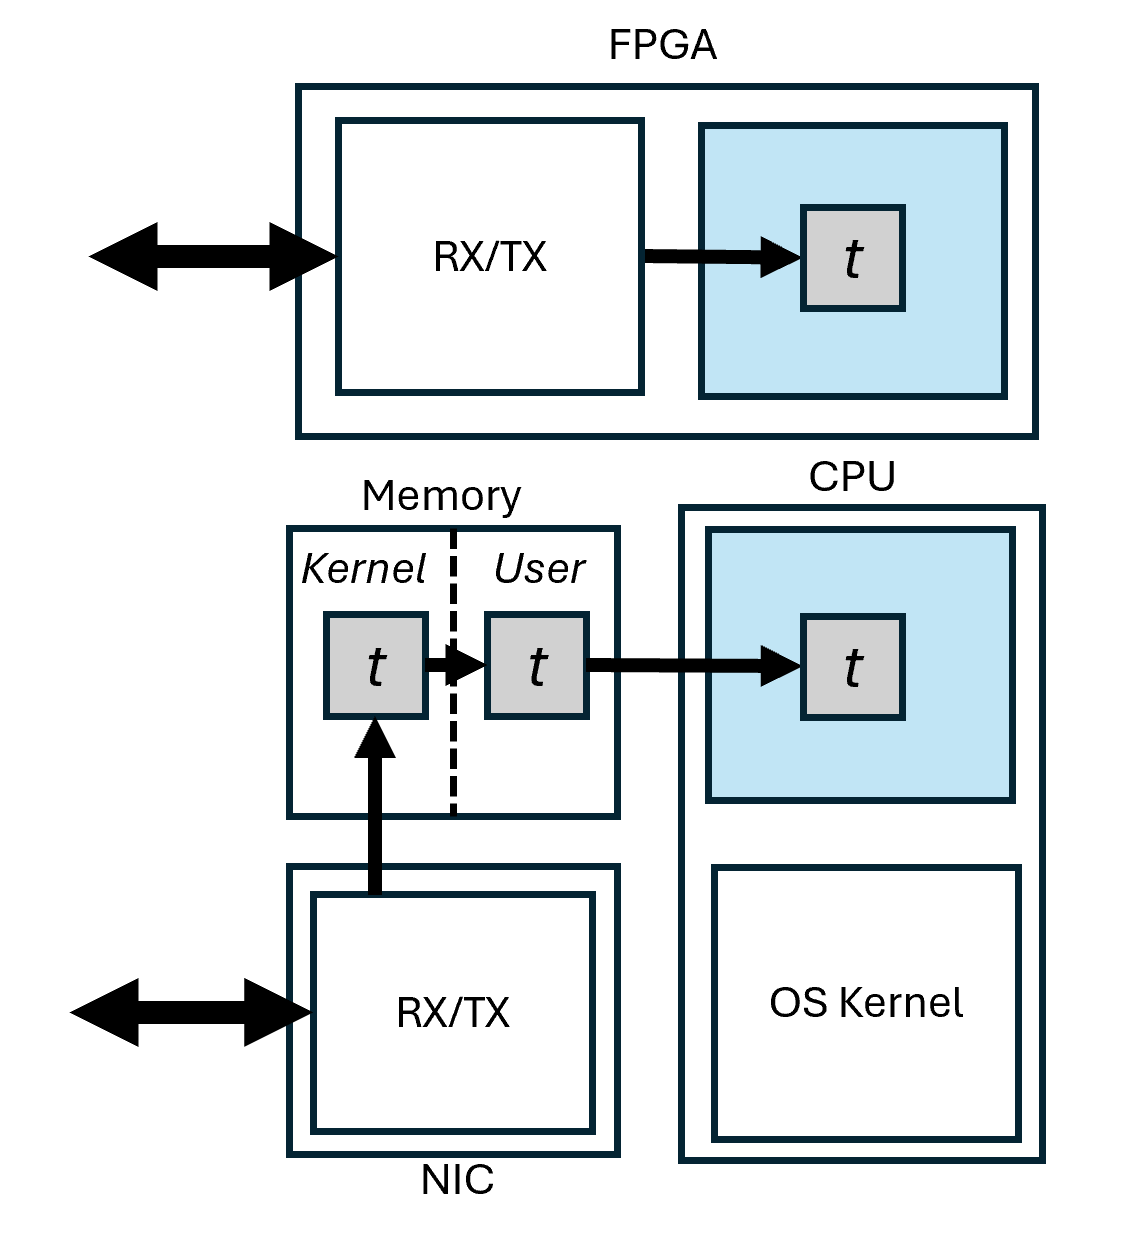
\includegraphics[width=0.5\linewidth]{Figures/Introduction/cpu-vs-fpga-network.png}
%     \caption{Caption}
%     \label{fig:placeholder}
% \end{figure}

\begin{figure}[t]
    \centering
        \begin{subfigure}{0.49\linewidth}
      \centering
      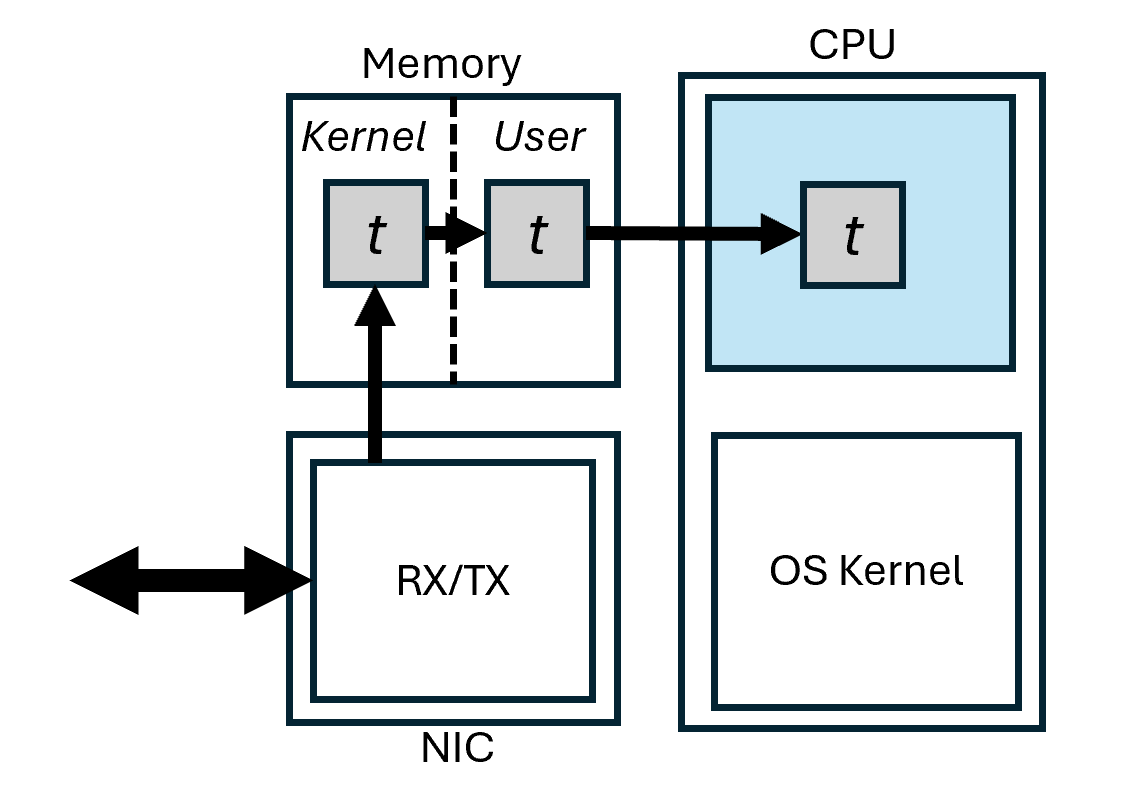
\includegraphics[width=\linewidth]{Figures/Introduction/cpu-network.png}
      \caption{CPU network interface via NIC and host memory.}
      \label{fig:cpu-network}
    \end{subfigure}
    \hfill
    \begin{subfigure}{0.49\linewidth}
        \centering
          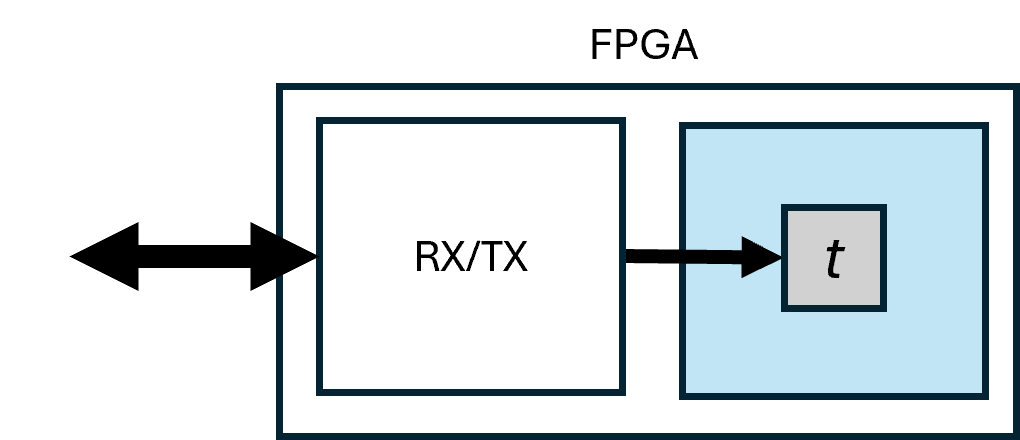
\includegraphics[width=\linewidth]{Figures/Introduction/fpga-network.png}
        \caption{FPGA configured as a SmartNIC with onboard accelerator.}
        \label{fig:fpga-network}
    \end{subfigure}
    \caption{A time series datapoint received by a traditional networked CPU (a) vs.\ an FPGA SmartNIC (b). The CPU path requires NIC$\to$PCIe$\to$kernel$\to$user-space copies; the FPGA transmits directly from network to accelerator.}
    \label{fig:cpuvsfpga}
\end{figure}
    
Two promising time series classification algorithms for acceleration are MiniRocket \cite{MiniRocket} and Hydra \cite{Hydra}. Both transform an input time series into a set of features that are classified using ridge regression or logistic regression, using convolutional kernels followed by a pooling layer which extracts the features. MiniRocket uses fixed ternary kernels ($\{-1, 2\}$) amenable to zero-DSP multiplication on FPGAs, while Hydra introduces learned random kernels with group-based histogram pooling, representing a complementary design point.

This paper presents FPGA accelerator architectures for MiniRocket and Hydra, evaluated in single-node and network streaming contexts. Key design contributions include dot-product reuse in the Convolution Engine, a fused convolution-pooling kernel eliminating intermediate storage, and a floating-point multiplier specialized to $\{-1, 2\}$ consuming zero DSP slices. MiniRocket achieves 8.5--58.7$\times$ speedup over optimized C++ with up to three compute units. At batch-size one, the 3-CU FPGA exceeds a Tesla T4 GPU on all datasets for both algorithms while consuming 2.1--2.6$\times$ less power. Both accelerators match reference CPU accuracy within 0.01\%.

